

\documentclass{beamer}
 
\usepackage[utf8]{inputenc}
\usepackage{tikz}
 
%Information to be included in the title page:
\title{El modelo de Potts aplicado a las neurociencias.}
\author{{Ángel Cáceres Licona}}
\institute{División de Ciencias Naturales e Ingeniería}
\date{2019}
 
 
 
\begin{document}
 
\frame{\titlepage}
 
\begin{frame}
\frametitle{Contenido}
\begin{itemize}
    \item El modelo de Ising
    \item El modelo de Potts como una generalización del modelo de Ising
    \item La analogía entre el cerebro y el modelo de Potts
    \item Predicciones del modelo
    \item Mediciones en el gusano C. Elegans.
  \end{itemize}
\end{frame}

\begin{frame}
\frametitle{El modelo de Ising}

%
El modelo de Ising es uno de los pocos modelos de part\'iculas interactuantes para el cu\'al se conoce una soluci\'on exacta. Es de gran utilidad ya que, aunque originalmente fue formulado para resolver problemas f\'isicos (ferromagnetismo) tiene much\'isima aplicaciones en el modelado de problemas de otras \'areas como la biolog\'ia, finanzas, etc.\\
\end{frame}

\begin{frame}
\frametitle{El modelo de Ising unidimensional}

En una dimensi\'on, el Hamiltoniano del modelo de Ising puede ser escrito como \\
%
\begin{eqnarray}
  \mathbb{H}=-\epsilon\sum_{i=1}^{N}\sigma_i\sigma_{i+1}-\mu B\sum_{i=1}^{N}\sigma_i \label{hamilIsing}
\end{eqnarray}

\end{frame}
\begin{frame}
\frametitle{El modelo de Ising}
%
donde $\sigma=\pm1$ y estos valores indican cada uno de los estados posibles: Si la part\'icula apunta hacia arriba o hacia abajo. Se usa tambi\'en la siguiente representaci\'on matricial:
%
\begin{eqnarray}
  |\uparrow\rangle &=&\begin{bmatrix}1\\0\end{bmatrix}\label{spinup},\\
  |\downarrow\rangle&=&\begin{bmatrix}0\\1\end{bmatrix}\label{spindown},
\end{eqnarray}
%
y se considera que la red es c\'iclica, es decir:
%
$$
\sigma_{N}=\sigma_{N+1},
$$
%
lo cual equivale a resolver el problema en un anillo.
%

\end{frame}

\begin{frame}
\frametitle{El modelo de Ising unidimensional}

\begin{figure}
\centering
\includegraphics[scale=0.5]{fig/Ising1D.png}
\caption{Modelo de Ising en una dimensión}
\end{figure}

\end{frame}

%
\begin{frame}
\frametitle{El modelo de Ising bidimensional}

Considere un enrejado bidimensional como el que se muestra

\begin{eqnarray}
  \begin{matrix}
  n+1 && \cdot && \cdot && \cdot && \cdot  \\
  \vdots && \cdot && \cdot && \cdot && \cdot  \\
  3 && \cdot && \cdot && \cdot && \cdot  \\
  2 && \cdot && \cdot && \cdot && \cdot  \\
  1 && \cdot && \cdot && \cdot && \cdot  \\
  1 && 2 &&   \dots&&  && n+1
  \end{matrix}, \nonumber
  \end{eqnarray}
\end{frame}
%


\begin{frame}
\frametitle{El modelo de Ising bidimensional}
Se imponen condiciones de frontera periódicas de forma que la part\'cula al final de cada fila y columna están conectadas. Esta configuraci\'on puede ser pensada como la superficie de un toro: 
%
\begin{figure}
\centering
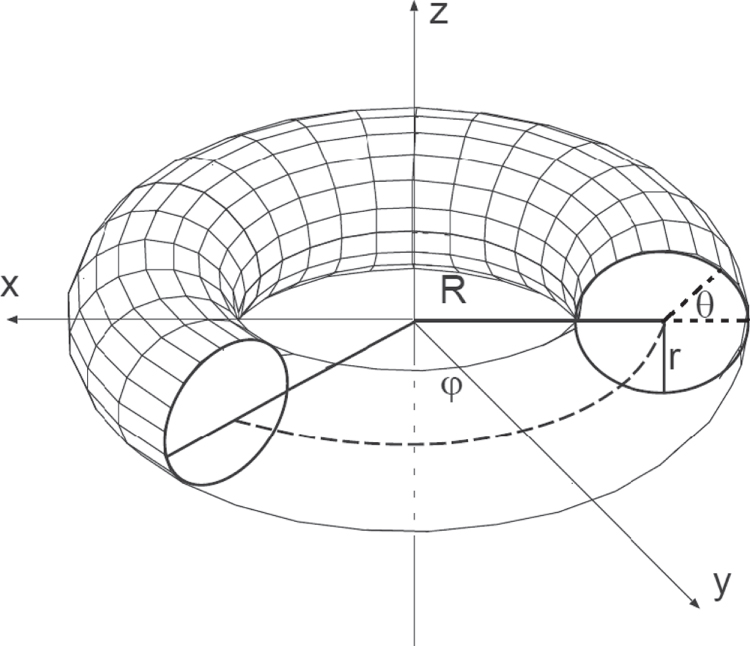
\includegraphics[scale=0.5]{fig/torus.png}
\caption{Modelo de Ising en dos dimensiones}
\end{figure}
\end{frame}

\begin{frame}
\frametitle{El modelo de Ising bidimensional}

El Hamiltoniano se escribe como 
\begin{eqnarray}
\mathbb{H}= -J \sum_{i,j} (\sigma_{i,j}\sigma_{i+1}+\sigma_{i,j+1}\sigma_{i,j}) - h \sum_{i,j}\sigma_{i,j},
\end{eqnarray}
donde los espines ahora son indexados por dos \'indices que corresponden a las coordenadas de un punto en el enrejado.

\end{frame}

\begin{frame}
\frametitle{El modelo de Ising bidimensional}
Una herramienta muy útil es el uso de simulaciones por computadora: 
%
\begin{figure}
\centering
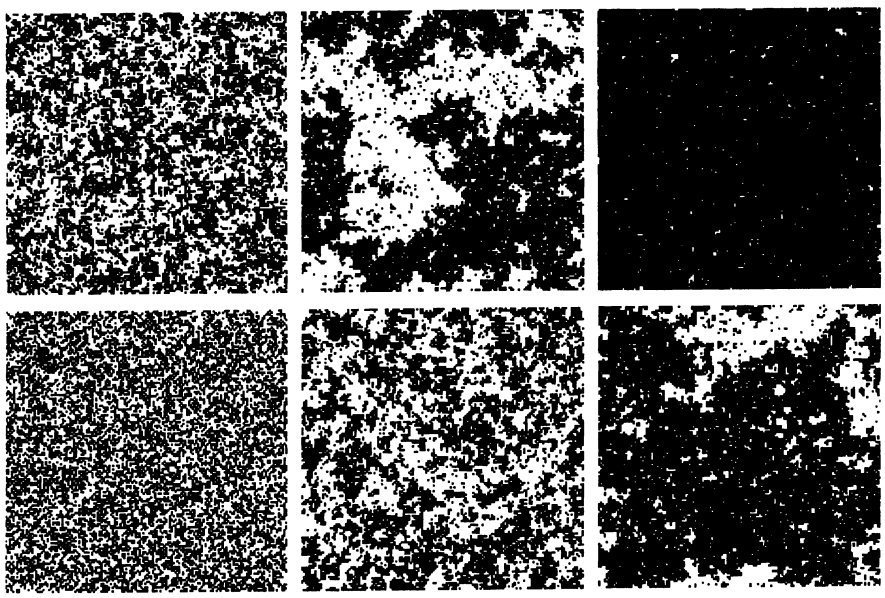
\includegraphics[scale=0.27]{fig/isingresult.png}
\caption{Simulacion de Montecarlo para el modelo de dos dimensiones}
\end{figure}

\end{frame}

\begin{frame}
\frametitle{El modelo de Potts}

El modelo de Potts es una generalización del modelo de Ising. 

\begin{figure}
\centering
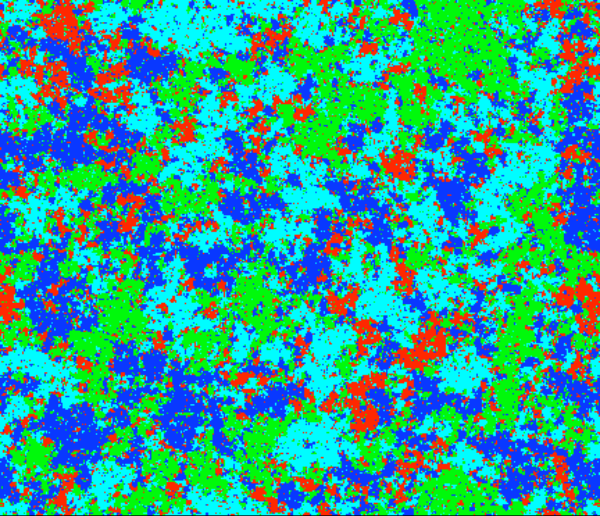
\includegraphics[scale=0.27]{fig/potts.png}
\caption{Simulacion de Montecarlo para el modelo de Potts}
\end{figure}
  

\end{frame}

\begin{frame}
\frametitle{La aplicación a las Neurociencias}
En este caso se estudia al gusano \textit{Caenorhabditis elegans}. Es un gusano que tiene 302 neuronas lo cuál hace muy sencillo su estudio. En este caso se limita al estudio de subconjuntos de 50 neuronas.

\begin{figure}
\centering
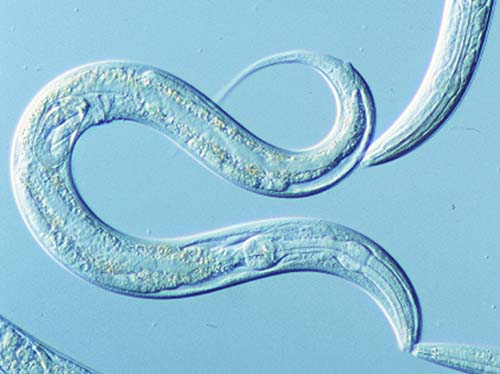
\includegraphics[scale=1]{fig/celegans.jpg}
\caption{El gusano \textit{Caenorhabditis elegans}}
\end{figure}

\end{frame}

\begin{frame}
\frametitle{La aplicación a las Neurociencias}

En este caso se usa una versión del modelo que tiene 3 estados: Subida, bajada y se mantiene. El Hamiltoniano de este sistema es el siguiente:
%
\begin{eqnarray}
  \mathbb{H}=-\frac{1}{2} \sum_{i \neq j}J_{i,j}\delta_{\sigma_i \sigma_j} - \sum_{i} \sum_{r=1}^{p-1}h_{r}^{i}\delta_{\sigma_{i}r}
\end{eqnarray}
%


\end{frame}

\begin{frame}
\frametitle{¿Funciona el modelo?}
\begin{figure}
\centering
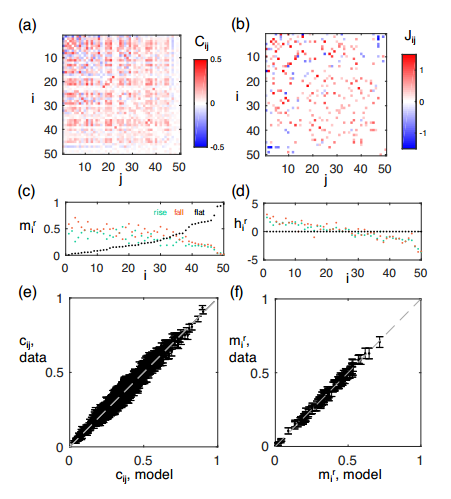
\includegraphics[scale=0.3]{fig/simulacioncelegans.png}
\caption{Simulaciones correspondiente al modelo para el gusano \textit{Caenorhabditis elegans}}
\end{figure}
\end{frame}


\begin{frame}
\frametitle{¿Funciona el modelo?}
\begin{figure}
\centering
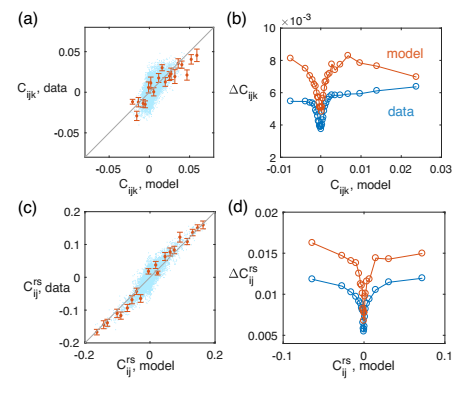
\includegraphics[scale=0.3]{fig/celeganscomparacion.png}
\caption{Simulaciones correspondiente al modelo para el gusano \textit{Caenorhabditis elegans}}


\end{figure}
\end{frame}
\begin{frame}
\frametitle{¿Funciona el modelo?}
\begin{figure}
\centering
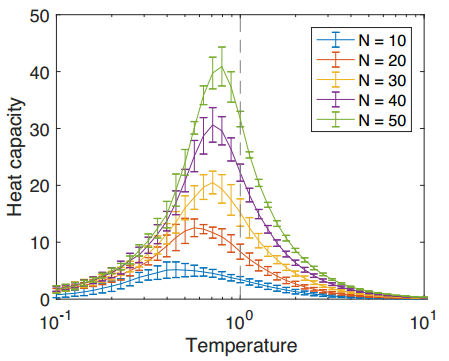
\includegraphics[scale=0.3]{fig/celeganstemperatura.png}
\caption{Simulaciones correspondiente al modelo para el gusano \textit{Caenorhabditis elegans}}


\end{figure}
\end{frame}
  
\begin{frame}
\frametitle{Referencias}

[1] L. Onsager, {\it Crystal statistics. I. A two-dimensional model with an order-disorder transition}, Physical Review, Series II, 65 (3–4): 117–149 (1944).\\

[2] P. M. Chaikin,  T. C. Lubensky, {\it Principles of Condensed Matter Physics,} First Edition, (Cambridge University Press, Cambridge, 1995).

[1] Xiaowen Chen, Francesco Randi, Andrew M. Leifer, y William Bialek1, {\it Searching for collective behavior in a small brain}, ArXiv e-prints,arXiv:1810.07623v1


\end{frame}


\end{document}